\section{Overall Architecture} \label{sec:Design-Architecture}

The design architecture defines the skeleton of the design of the program, and is highly influenced by the applied design patterns: MVC and IoC. 

Following the MVC mindset, the skeleton must have a clear division between the presentation layer, the data structure and the actions between the two. Also by the IoC mindset, we must keep an all-purpose core, which extends into custom, and more specialised modules.\footnote{Here modules are used in the general sense, and not just confined to the F\# modules}

If we start by looking at the core, we will have an entity responsible for the main window. This entity will have a presentation layer and means of overall navigation between the modules within the main window. Also, there will be no functionality to interact with the model - this will be reserved for specialised sub-modules. 

The core of the program, as defined here, will be referenced as the 'main window', to make it clear where its responsibility lies.

A crucial part of the MVC design pattern is to have a model completely detached from the view, which comes naturally using this setup, since the model will be accessible from multiple modules, and interacted with using defined procedures. The main window, with the model-view-control division can be seen in figure \ref{fig:Architecture-MainWindow}.

\begin{figure}[H]
    \centering
    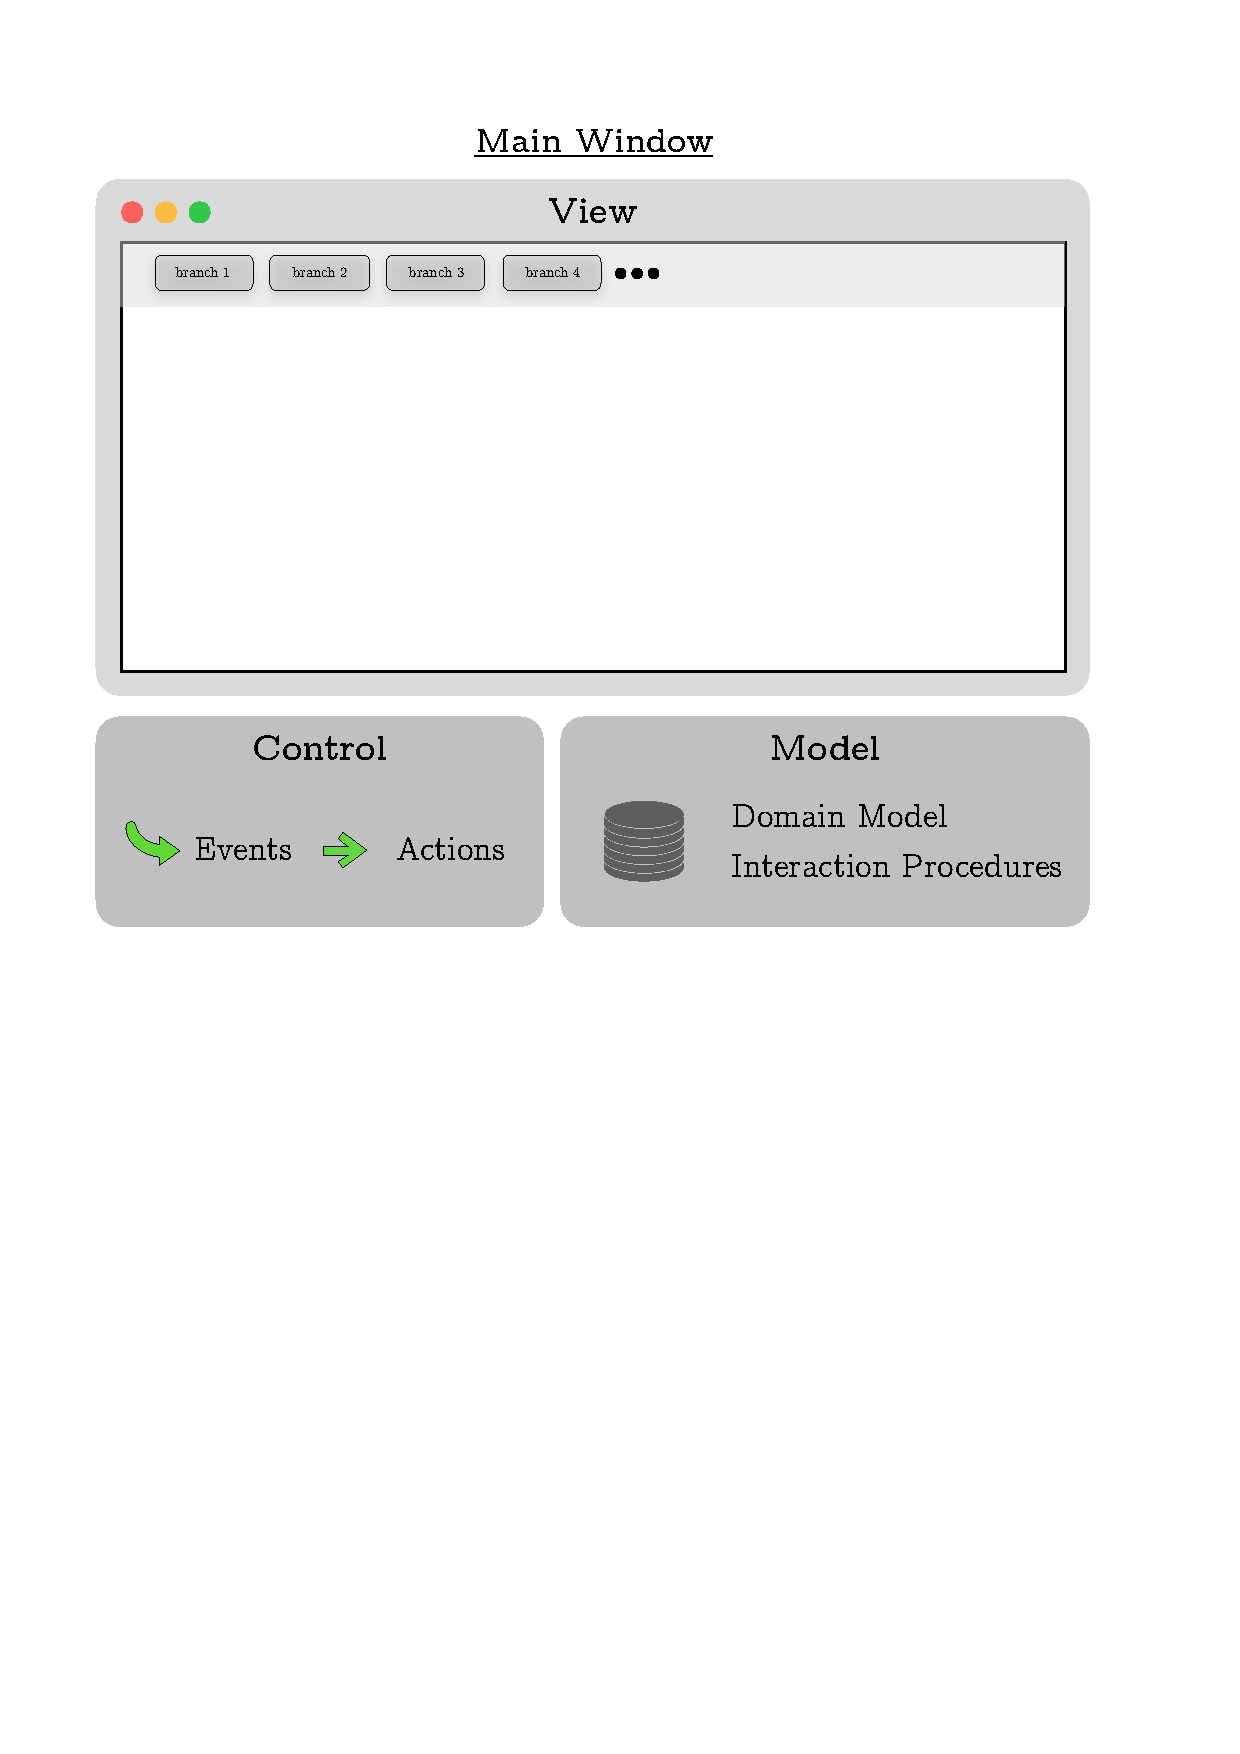
\includegraphics[page = 1, width = 0.6\linewidth]{.Figures/Architecture.pdf}
    \caption{Main window for the program, following the model-view-control design pattern. Responsible for overall navigation, without any specific functionality regarding model interaction/manipulation.}
    \label{fig:Architecture-MainWindow}
\end{figure}

If we take a look at the main parts of the program again, we have the model extraction, the impact computation and some way of viewing the indicator scores for the system. These divide suitable up into different modules from/inside the main window, each with their individual views and controls. This structure follows naturally from the IoC design pattern, and because of the resemblance of a tree, we will call the sub-modules 'branches'. This way we can also avoid any confusion between architectural modules and F\# modules.

When we look at the model, the three parts of the program either create or utilise information stored in the data structure. Therefore it would be beneficial to distribute a reference to the same model throughout the different branches, and let them either alter the data during model extraction, or access the final composed data structure during computation and visualisation.

A branch will then have a MVC structure as seen in figure \ref{fig:Architecture-Branch}.

\begin{figure}[H]
    \centering
    \includegraphics[page=2, width=0.6\linewidth]{.Figures/Architecture.pdf}
    \caption{A generic branch for the program, intended to function inside the main window, following the model-view-control design pattern. The branch accesses the model through a reference handed to it during initialisation. This is visualised by opaqueness and a perforated boarder.}
    \label{fig:Architecture-Branch}
\end{figure}

With these architectural components, we can construct a tree, with the main window as the root, with the individual branches, as seen in figure \ref{fig:Architecture-Tree}. Each branch can subsequently, and recursively extend into branches, if any special task benefits from it. 

\begin{figure}[H]
    \centering
    \includegraphics[page=3, width=0.9\linewidth]{.Figures/Architecture.pdf}
    \caption{The architecture in form of a tree of abstract components. Each component follows the model-view-control design pattern, while the tree itself follows utilises inversion of control.}
    \label{fig:Architecture-Tree}
\end{figure}

The overall architecture can then be summed up, as a tree with complexity and specificity proportional to the depth of the tree, where each node of the tree (internal and leaf) are comprised according to the model-view-control, but with a global model dispersed from the root.

\vspace{1cm}
We will now look at each of the main parts individually, focusing on how they can be designed using the defined branches.